\chapter{Exploration 2: extending XIMPEL for playing media types concurrently}
\label{chap:exploration2}
%no conlclusion in his thesis on how HTML 5 influences hypermedia
I read Stefan Bruins his thesis over and over. While a thesis is academic, I detected a form of sadness in it, a regret perhaps. There was a longing to play media items in parallel. Everything was set for it: the architecture expected it, in Stefan his thesis it was written about and because of the command-line tutorial, I needed it. However, it was not there.

At the time I did not think much of it, but at the end of my thesis I realized that parallel media playback and parallel media items interfacing with applications is a topic of research for computer scientists that could provide new insights into the nature of computation and human-computer interaction. Moreover, parallel media playback from a hypermedia standpoint is inevitably linked with multiple time lines. Because of this it has some resemblance to time travel. It is even possible to have a poor man's simulation of time travel with parallel media playback! But let's visit this topic in the future.

% Note to self: Stefan geeft geen justification voor parallel media playback, daarnaast geeft het twee tips
% Doe het via de media player
% Doe geen nested parallel tags
% Ook hier geeft hij geen justification voor
Let's start from the beginning: Bruins explored in his thesis whether XIMPEL could be ported to the web without the use of plugins like it was programmed in the past (with the Flex SDK, As3 and Flash). In other words could it be ported to the web with: HTML5, CSS and JavaScript? The answer was a resounding yes \cite{stefan2016}. Bruins also suggested future work to be done on the XIMPEL platform. One of the most prominent examples is the creation of a parallel media player. XIMPEL has been architected with a parallel media player in mind. Therefore, programming a parallel media player will give an even more conclusive answer to his research question of how one can be programmed. Furthermore, implementing a parallel media player will allow us to have a closer look at possible technical difficulties regarding HTML5 and attempting to play multiple videos in sync. 

On another note, creating a parallel media player gives much more insight as to what hypermedia is. Simply creating a framework that plays one media element at the time is a rather limited experience in the form of hypermedia. Creating a parallel media player for XIMPEL would mean that more video and audio and custom media types could be played (note: it was already possible to display multiple images and text via the overlay mechanism and there was iframe support). Parallel media playback is possible in SMIL since version 1.0. However, SMIL and other hypermedia frameworks does not seem to offer a plugin like extensibility which means that the implications of parallel media playback and application media types (e.g. `<terminal>`) are left unexplored. %no ref -- too much work


\section{Architecture of parallel playback}

By looking at the architecture of XIMPEL and how the sequence player was implemented, implementing a prototype of the parallel player has been more doable than without it. However, there were a couple of caveats in the original architecture of XIMPEL as stated in Bruins thesis (see figure \ref{fig:original_architecture}). First of all, the figure suggests that a `SequencePlayer` is able to play another `SequencePlayer`. After testing the following playlist (see playlist \ref{playlist:sequenceplayers_wrong}) this is demonstrably false. Fortunately, it is false because there is no need for a `SequencePlayer` playing yet another `SequencePlayer` that will then play media types in sequence. The reason is: one `SequencePlayer` already plays media types in sequence!

\begin{lstlisting}[language=XML, caption=This playlist contains a nested sequence tag and therefore does not work. This demonstrates that the architecture in figure \ref{fig:original_architecture} as outlined in Stefan Bruins\cite{stefan2016} his thesis (fortunately) does not work as prescribed., label=playlist:sequenceplayers_wrong]
<ximpel>
<config>
    <enableControls>true</enableControls>
    <controlsDisplayMethod>overlay</controlsDisplayMethod>
</config>
<playlist>
    <subject id="lesson1">
        <sequence>
            <sequence>
                <message text="hey" />
            </sequence>
        </sequence>
    </subject>
</playlist>
</ximpel>
\end{lstlisting}

\begin{lstlisting}[language=XML, caption=this playlist does work and serves as a counter example to playlist \ref{playlist:sequenceplayers_wrong} which has a nested sequence tag., label=playlist:sequenceplayers_right]
<ximpel> 
<config>
    <enableControls>true</enableControls>
    <controlsDisplayMethod>overlay</controlsDisplayMethod>
</config>
<playlist>
    <subject id="lesson1">
        <sequence>
            <message text="hey" />
        </sequence>
    </subject>
</playlist>
</ximpel>
\end{lstlisting}

The current architecture has been updated to reflect the implemented changes as well as the intention of XIMPEL (see figure \ref{fig:architecture}). In its current architecture the XIMPEL player always calls \textit{the} `SequencePlayer`. And a `SequencePlayer` can either call a `ParallelPlayer` or a `MediaPlayer`. A `MediaPlayer` plays a `MediaType` (e.g. video or audio). A `ParallelPlayer` plays multiple `SequencePlayer`s. By doing it this way it is possible to allow nesting of parallel tags. In some cases nested parallel tags is desirable since at every level of the multimedia presentation an author will able to decide which parts of the presentation have to play in parallel and which parts of the presentation have to play in sequence.

These players have corresponding models. So a `SequencePlayer` plays a `SequenceModel`, a `ParallelPlayer` plays a `ParallelModel` and a `MediaPlayer` plays a `MediaModel`. From `MediaModel`s, `MediaType`s are constructed.

The extensibility of XIMPEL and playing media types in parallel allows for one unexpected idea: one can extend XIMPEL with applications that are not multimedia. This question has been explored in another part of this thesis (see chapter \ref{chap:exploration1}).

\begin{figure}
\centering
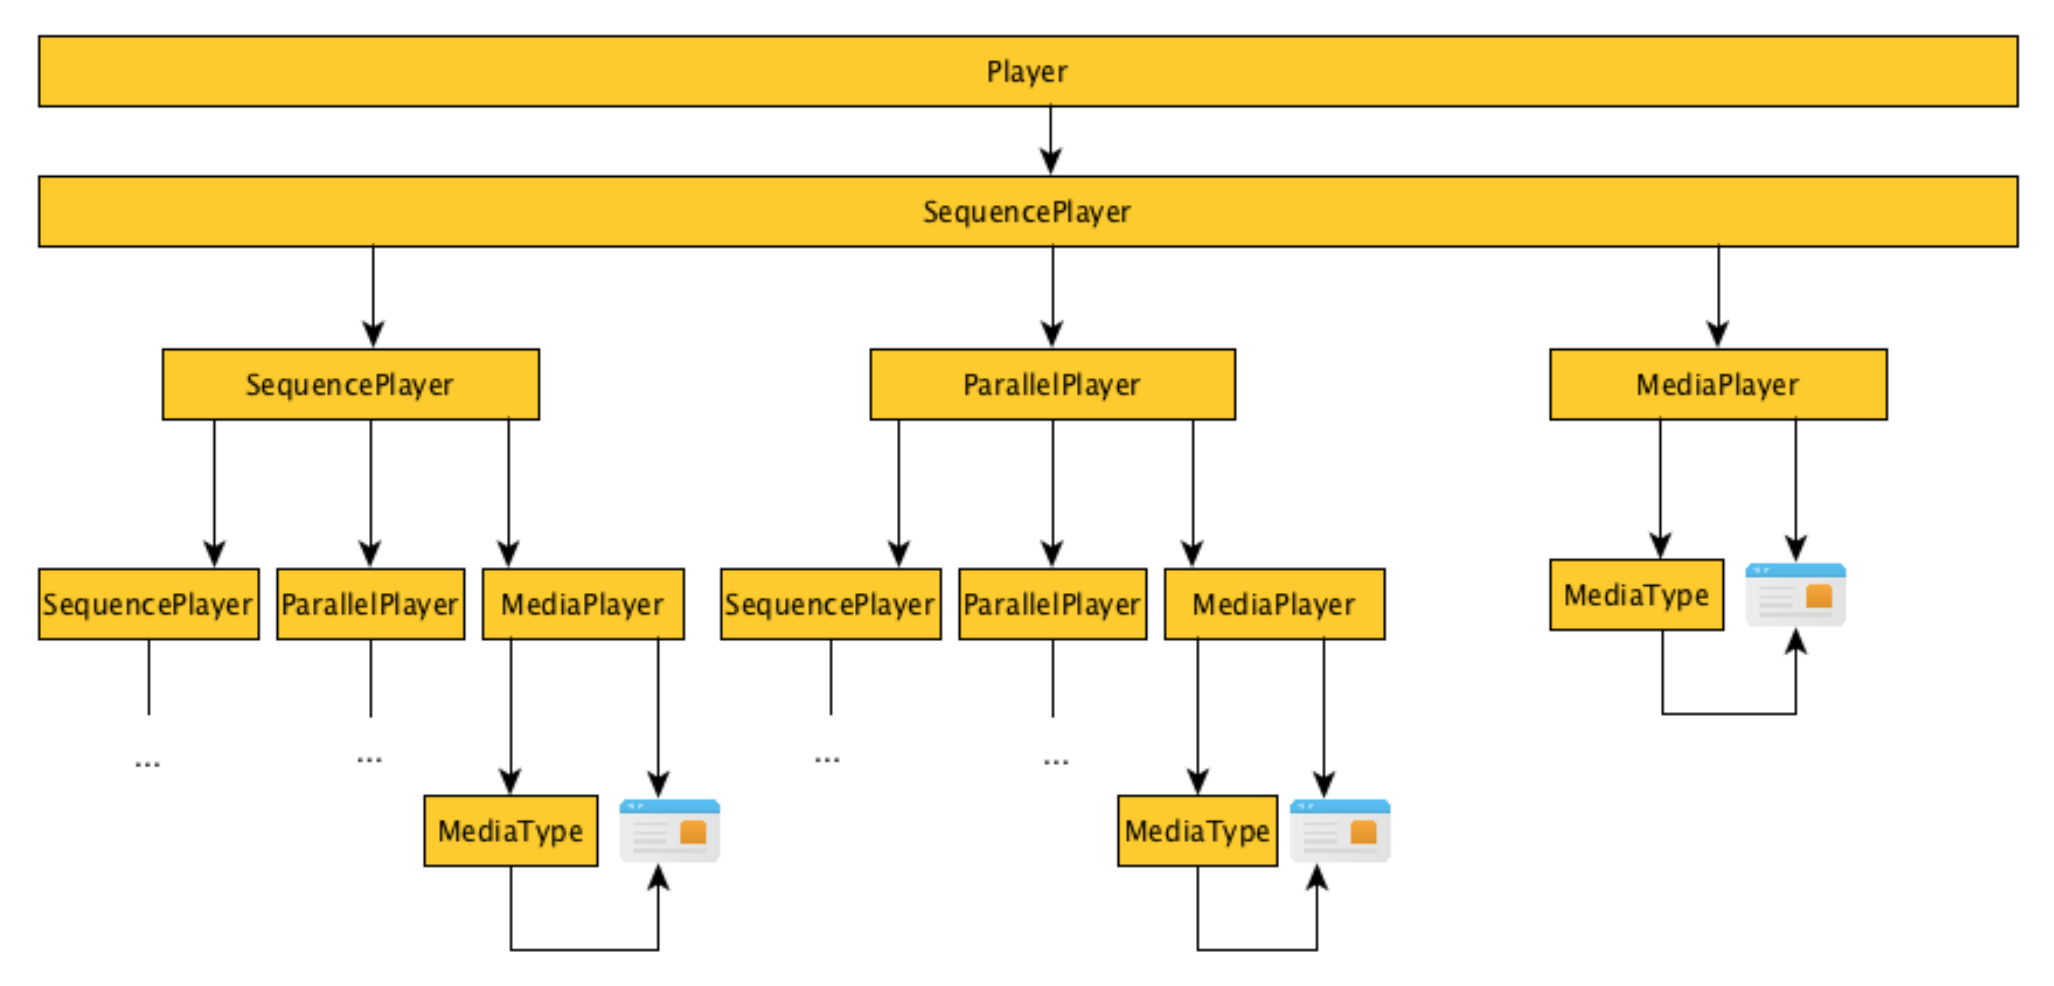
\includegraphics[width=1.35\textwidth, center]{ximpel_original_player_architecture.png} % quotation marks make sure file name does not display
\caption{The original player architecture of XIMPEL. The media type gives rise to media which can be: video, audio, image, text or a custom defined media type. This architecture has been proposed and (partially) implemented by Stefan Bruins \cite{stefan2016}. It has been demonstrated by me that nested SequencePlayers have not been implemented and I also explained why this does not need to happen in the beginning of this chapter. The diagram shows the possible valid children a player would be able to play.}
\label{fig:original_architecture}
\end{figure}

\subsection{Implementation of parallel playback}
For the architecture of any player in XIMPEL (e.g. a parallel, sequence or media player) there is a pipe line. (1) It starts with parsing the XIMPEL playlist, which is in XML. (2) The data parsed by the XML syntax get put into an in-memory configuration object, which holds the details of the XIMPEL playlist. (3) The player itself uses, in most cases, a subset of the in-memory configuration object\footnote{Since the whole object is the complete playlist, so a part of the in-memory memory object it is the relevant part of the playlist that needs to be played}. Each individual part of the pipe line is explained in its own section.

\subsubsection{The parallel player and parsing}
The first part of implementation that needed to be programmed was the parser. The parallel player needed to be registered as a valid child, since it otherwise would refuse to parse the `<parallel>` tag. In the `processSubjectNode` method the `processParallelNode` method is called which will return a parallel model which is part of the in-memory configuration object. The method will determine the info of the `<parallel>` tag (e.g. its parent and children) which is needed to loop through its children. While looping through its children, the method will determine whether this particular `<parallel>` tag has: `<sequence>` tags, `<media>` tags or custom defined media type tags. It will then add those to the parallel model.

\subsubsection{The in-memory configuration of the parallel player}
The `ParallelPlayer` uses a `ParallelModel`. The `ParallelModel` itself is nothing more but a glorified array, as of now. It has a property called `list`. It also has a method called `add`, which means: add the children of the `<parallel>` tag to this list. These children are wrapped in a `SequenceModel` since it is one `SequencePlayer`, managing one media item. It furthermore inherits the `get` and `set` method from `ximpel.Model`. The methods and variables in every method are completely identical to the `SequenceModel`. It only differs from the `SequenceModel` with the idea that the playing order of the `ParallelModel` is to play everything at once, instead of in a default or random sequential order. 

\subsubsection{The parallel player itself}
The major code revisions were regarding the `SequencePlayer` and creating the `ParallelPlayer` itself. XIMPEL always has a top `SequencePlayer` (i.e. \textit{the} `SequencePlayer`), it needs to be aware of how to start a `ParallelPlayer`. For example, when the `SequencePlayer` needs to stop it also needs to stop the `MediaPlayer` and the `ParallelPlayer`. Another example is that there needs to be a method in the `SequencePlayer` to play a `ParallelModel`. All the method really does is passing it on to the actual `ParallelPlayer`, but the `SequencePlayer` still needs to know about it.

%Should I apply variable modifiers?

The implementation of the `ParallelPlayer` itself is inspired by the `SequencePlayer`. Unlike the `SequencePlayer` which plays media types in sequence, the idea is to play everything all at once. The architecture of XIMPEL already allows for players to start playback for other players. In the architecture outlined in figure \ref{fig:architecture}}, a `ParallelPlayer` will have multiple players as its children of some kind. 

As possible candidaties, one could consider the `ParallelPlayer` to have multiple `MediaPlayer`s, or multiple `SequencePlayer`s, or a custom implementation of multiple players. For sake of simplicity I chose that the `ParallelPlayer` is able to have multiple `SequencePlayer`s, simply for the reason that a `SequencePlayer` is a wrapper for a `MediaPlayer`. Because it is a wrapper, it has the same and extended functionality. This extended functionality was eventually needed when I realized later on that you might want to have a sequence while you are playing something parallel. This is entirely possible with multiple `SequencePlayer`s, but it would be more tricky to create with multiple `MediaPlayer`s.

For all the other functionalities the core idea of the `ParallelPlayer` is that all `SequencePlayer`s need to be: played, stopped, paused or resumed. In other words: everything a normal `SequencePlayer` does, a `ParallelPlayer` does too but then for multiple `SequencePlayer`s. The diagram below shows the new architecture of XIMPEL on a high level including the newly implemented `ParallelPlayer` (see figure \ref{fig:architecture}).

\section{Conclusion}
A conclusion on such a technical subject as this is fairly straightforward: parallel media playback works and no issues have been observed as of yet. Other designs were possible but they have not been investigated. On another note, the creation of the parallel player allows for parallel playback, which allows the terminal media type of exploration 1 to be used in a much more useful manner since it is now possible to add video playback with it. Parallel playback allows for multiple media items of the same or different media types to complement each other through the ways such media items present their information.

However, such a conclusion is too short to be satisfying. Moreover, since this thesis is an explorative one it may be fruitful to know how far we have come. So in the remainder of the conclusion we are going to take a step back.

% what is the relationship between XIMPEL and education? And how does XIMPEL need to be improved for it to better serve education? 
Since exploration 1, I started with the question of how XIMPEL and education relate and how it needs to be improved, I now stumbled upon a new question. What are the implications of parallel media playback? It is mostly the latter question that will be answered in the remainder of these pages. This is not because I wanted to answer it, it is because I stumbled upon many questions and issues going forward with parallel media playback. 

Let us look in the future regardless. The `ParallelPlayer` has a lot of implications such as the user need for a media item surviving a subject switch (MISSS) when a user jumps to a new subject (see exploration 6) or the implications for time scrubbing are so numerous that it poses serious design issues (see exploration 5). The biggest implication of all is that everything is a lot less complicated when the developer only has one playing media item at a time to worry about instead of as many as a `ParallelPlayer` allows. Currently, XIMPEL is now able to play playlist \ref{playlist:example_playlist}, which is in appendix \ref{chap:exploration2_appendix}, which means it is able to play parallel media.
% Note that the media and sequence tags can be interchangeably used. 

Let us look to the next exploration. Exploration 1 sparked exploration 3. So for the next exploration, ideas about parallel media playback will be left alone. These ideas come back in exploration 5 and 6. So dear reader, I now give you a choice. Explorative reading is an art in itself as well.

\textbf{Option A:} You can either start reading exploration 5 and 6 if you want to know more about parallel media playback.

\textbf{Option B:} Or, you can start reading exploration 3 and read how I recreate the majority of XIMPEL to ReactJS.

The choice itself centers around the following question: do you want to thematically read all the themes in such a way that it is easier to digest? Choose option A. Do you want to read how the thesis happened in chronological order? Choose option B. Regarding option A, it is my suggestion to read the thesis in the order of: exploration 5, exploration 6, exploration 4 and exploration 3. Exploration 3 and 4 could be swapped since it is exploration 1, 2, 5 and 6 that are thematically linked. Regarding option B, I would like to remind the reader that the correct chronological order of how the explorations have been done are: exploration 3 (read only until the first subsection), exploration 4 to 6 and back to the rest of exploration 3. 

% Maybe in exploration 1?
% Another implication pertaining to parallel playback and one that has been shown in exploration 1 is that it allows a XIMPEL author to play multiple media items on one page. One use case for that is education, which benefits from playing multiple media items regarding course creation. The odd fact has been observed that some media items are not items of media but rather applications disguised as media items. This seems strange, but it works. The strangeness might be because the philosophy of hypermedia in general has been formulated when the view of the web as a hypertext document was still in vogue. In 2018, the idea of a website as an application is a lot more trending\cite{garrett2000, paulson2005}. 

% Jesse James Garrett wrote in 2000 about it and stated:``The Web was originally conceived as a hypertextual information space; but the development of increasingly sophisticated front- and back-end technologies has fostered its use as a remote software interface. This dual nature has led to much confusion, as user experience practitioners have attempted to adapt their terminology to cases beyond the scope of its original application.\cite{garrett2000}'' He saw a clear difference between the web as software interface and the web as hypertext system. Five years later an industry trends article appeared titled \textit{Building Rich Web Applications with Ajax} in the peer-reviewed IEEE Computer Society in which they shed more light on this trend, through the help of Garrett his visual image\cite{paulson2005}.

% One could ask: since the philosophy of the web shifted, how should the philosophy of XIMPEL react to it? Should it stay the same? Or should it adapt? The concepts of hypermedia have not been updated with this paradigm shift about the web. If the philosophy of hypermedia adapts, then it may be possible to reconcile the whole media versus non-media paradox regarding the extensibility of XIMPEL. While this question is not an implication of parallel media playback, the process of creating the parallel media player did trigger it.


\begin{figure}
\centering
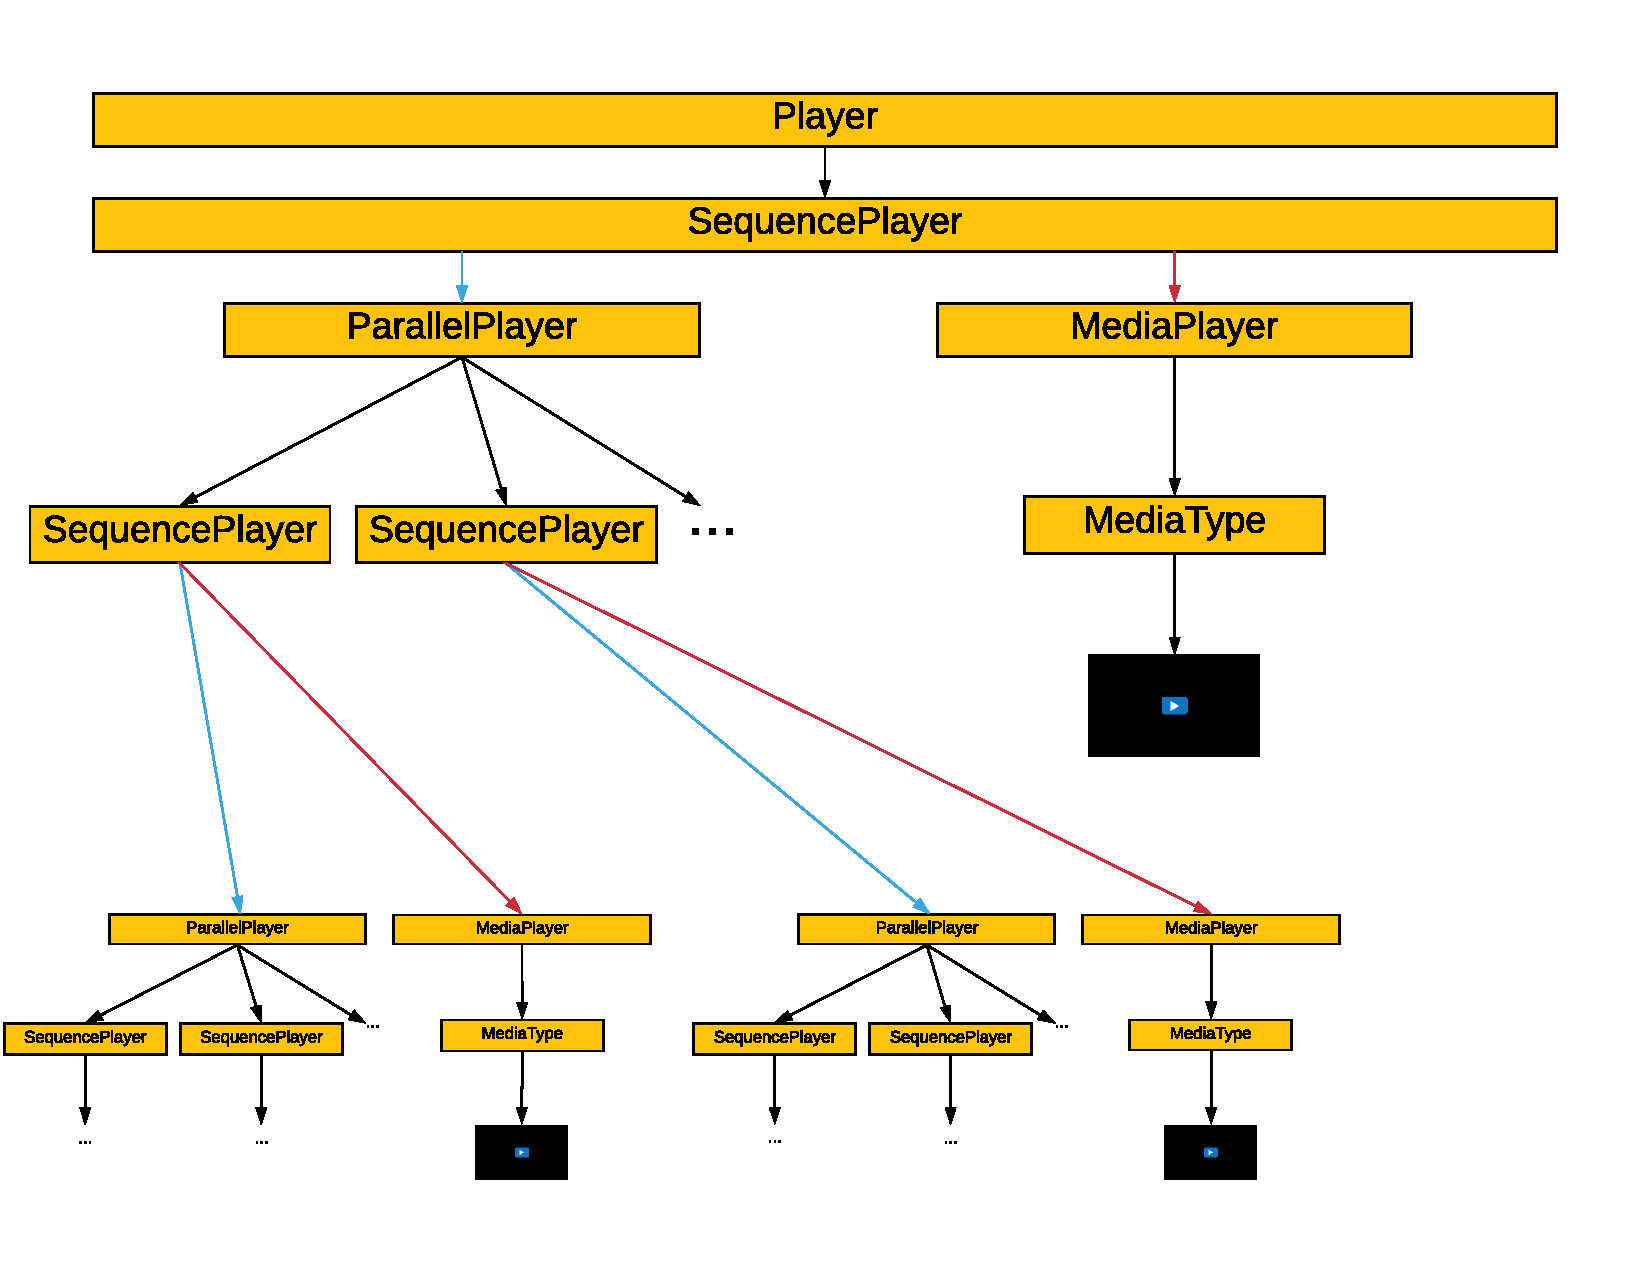
\includegraphics[width=1.35\textwidth, center]{ximpel_player_architecture.pdf} % quotation marks make sure file name does not display
\caption{The current player architecture of XIMPEL. The media type gives rise to media which can be: video, audio, image, text or a custom defined media type. The diagram shows which possible players can be played but also how many players another player can play. A blue or red line indicate that the player of which the line originates needs to choose between one of them. A black line means that a player will be invoked by another player.}
\label{fig:architecture}
\end{figure}


